%%%%%%%%%%%%%%%%%%%%%%%%%%%%%%%%%%%%%%%%%
% University/School Laboratory Report
% LaTeX Template
% Version 3.1 (25/3/14)
%
% This template has been downloaded from:
% http://www.LaTeXTemplates.com
%
% Original author:
% Linux and Unix Users Group at Virginia Tech Wiki 
% (https://vtluug.org/wiki/Example_LaTeX_chem_lab_report)
%
% License:
% CC BY-NC-SA 3.0 (http://creativecommons.org/licenses/by-nc-sa/3.0/)
%
%%%%%%%%%%%%%%%%%%%%%%%%%%%%%%%%%%%%%%%%%

%----------------------------------------------------------------------------------------
%	PACKAGES AND DOCUMENT CONFIGURATIONS
%----------------------------------------------------------------------------------------

\documentclass{article}

\usepackage[a4paper, total={6in, 9in}]{geometry}

\usepackage{siunitx} % Provides the \SI{}{} and \si{} command for typesetting SI units
\usepackage{graphicx} % Required for the inclusion of images
\usepackage{amsmath} % Required for some math elements 
\usepackage[italian]{babel}
\usepackage{booktabs}% Better table spacing
\usepackage{subcaption}
\usepackage{tikz}
\usepackage{pgfplots}

\setlength\parindent{0pt} % Removes all indentation from paragraphs

\renewcommand{\labelenumi}{\alph{enumi}.} % Make numbering in the enumerate environment by letter rather than number (e.g. section 6)

%\usepackage{times} % Uncomment to use the Times New Roman font

\usepackage{tikz}
\usetikzlibrary{positioning}
\tikzset{%
  every neuron/.style={
    circle,
    draw,
    minimum size=1cm
  },
  neuron missing/.style={
    draw=none, 
    scale=4,
    text height=0.333cm,
    execute at begin node=\color{black}$\vdots$
  },
}

%----------------------------------------------------------------------------------------
%	DOCUMENT INFORMATION
%----------------------------------------------------------------------------------------

\title{Rete neuronale per Ising e XY} % Title

\author{Martina \textsc{Crippa}, Pietro Francesco \textsc{Fontana}} % Author name

\date{\today} % Date for the report

\begin{document}

\maketitle % Insert the title, author and date

%\begin{center}
%\begin{tabular}{l r}
%Date Performed: & January 1, 2012 \\ % Date the experiment was performed
%Partners: & James Smith \\ % Partner names
%& Mary Smith \\
%Instructor: & Professor Smith % Instructor/supervisor
%\end{tabular}
%\end{center}

% If you wish to include an abstract, uncomment the lines below
% \begin{abstract}
% Abstract text
% \end{abstract}

%----------------------------------------------------------------------------------------
%	SECTION 1
%----------------------------------------------------------------------------------------

\section{Introduzione}
Alcuni sistemi fisici presentano diverse fasi e al variare della temperatura transiscono da una fase all'altra. La temperatura a cui avviene questo passaggio di fase viene detta temperatura critica. In generale la transizione di fase è descritta da un parametro d'ordine, ad esempio la magnetizzazione nel modello di Ising. L'obiettivo del progetto è implementare e studiare una rete neuronale in grado di apprendere il parametro d'ordine e quindi classificare correttamente la fase di diverse configurazioni di un sistema, individuando infine la temperatura critica. Successivamente si è provato ad eseguire una procedura analoga nel caso di un sistema che non presenta una transizione di fase descrivibile attraverso un parametro d'ordine, quindi dove la rete neuronale apprende altre caratteristiche del sistema per classificarne la fase.
Il lavoro prende spunto da diversi articoli pubblicati negli ultimi due anni che affrontano la stessa tematica \cite{carrasqu,melko,wessel}.

%----------------------------------------------------------------------------------------
%	SECTION 2
%----------------------------------------------------------------------------------------

\section{Sistemi fisici e simulazioni}
In questo lavoro sono stati simulati e studiati due sistemi matematici su reticolo bidimensionale:  il modello di Ising e il modello XY.
\subsection{Modello di Ising}
Il modello di Ising descrive il comportamento di spin su reticolo che possono assumere valori $\{+1;-1\}$ interagendo tra loro. L'hamiltoniana di interazione che è stata utilizzata in questo lavoro è
\begin{equation}
H=- \sum_{\langle i~j\rangle} \sigma_i\sigma_j
\end{equation} 
dove le parentesi angolari indicano l'interazione a primi vicini fra gli spin. L'energia di interazione è costante fra tutti gli spin e posta pari a $1$. Ad alte temperature il contributo entropico fa si che il sistema si trovi in uno stato di disordine, ovvero nella fase paramagnetica \ref{fig:isingP}. Abbassando la temperatura prevale il contributo energetico quindi al di sotto della temperatura critica gli spin tendono ad allinearsi e il sistema transisce alla fase ferromagnetica \ref{fig:isingF}: tale transizione di fase è detta del \emph{secondo ordine}.
\begin{figure}[h]
\centering
\begin{subfigure}[b]{0.4\linewidth}
\centering
\begin{tikzpicture}[> = stealth, scale=0.8]
\draw[gray,dashed,step=1.5cm] (-1,-1) grid +(5cm,5cm);
    \foreach \y in {0,1,2} 
        \foreach \x in {0,1,2}
            \node[shape = rectangle, minimum width = 0.75cm, minimum height = 0.75cm] (dot_\y_\x) at (1.5*\x,1.5*\y){};
    
   \draw[ultra thick,blue, ->]  (dot_0_0.south) -- (dot_0_0.north);
   \draw[ultra thick,red, ->]  (dot_1_1.south) -- (dot_1_1.north);
   \draw[ultra thick,red, ->]  (dot_2_1.south) -- (dot_2_1.north);
   \draw[ultra thick,blue, ->]  (dot_1_2.south) -- (dot_1_2.north);
   \draw[ultra thick,red, ->]  (dot_2_2.south) -- (dot_2_2.north);
   \draw[ultra thick,red, ->]  (dot_0_2.south) -- (dot_0_2.north);
   \draw[ultra thick,blue, ->]  (dot_2_0.south) -- (dot_2_0.north);
   \draw[ultra thick,blue, ->]  (dot_0_1.south) -- (dot_0_1.north);
   \draw[ultra thick,red, ->]  (dot_1_0.south) -- (dot_1_0.north);
\end{tikzpicture}
\caption{Paramagnetico} \label{fig:isingP}  
\end{subfigure}
\begin{subfigure}[b]{0.4\linewidth}
\centering
\begin{tikzpicture}[> = stealth, scale=0.8]
\draw[gray,dashed,step=1.5cm] (-1,-1) grid +(5cm,5cm);
    \foreach \y in {0,1,2} 
        \foreach \x in {0,1,2}
            {\node[shape = rectangle, minimum width = 0.75cm, minimum height = 0.75cm] (dot_\y_\x) at (1.5*\x,1.5*\y){};
            \draw[ultra thick,blue, ->]  (dot_\y_\x.south) -- (dot_\y_\x.north);}
\end{tikzpicture}
\caption{Ferromagnetico} \label{fig:isingF}  
\end{subfigure}
\caption{Ising 2D}
\end{figure} 
Il parametro d'ordine che evidenzia la transizione di fase è la magnetizzazione totale del sistema:
\begin{equation}
M=\sum_i \sigma_i
\end{equation}
Sono stati studiati sistemi con geometrie di reticolo differenti e conseguentemente aventi un numero di primi vicini (nn) e temperatura critica divera, i cui valori sono riportati in tabella \ref{tab:ltI}.
\begin{table}[h]
\begin{center}
\begin{tabular}{lllll}
\toprule
reticolo & nn & $T_c$ & $T_c$ approx $[$\si{K}$]$ & $T_{init}$ $[$\si{K}$]$\\
\midrule
quadrato & $4$ & $2/ \!\ln{(1+\sqrt{2})}$ & $2.2692$ & $1.0$\\
triangolare & $6$ & $4/\!\ln{3}$ & $3.6410 $ & $2.0$\\
honeycomb & $3$ & --- & $1.5187$ & $0.0$\\
\bottomrule
\end{tabular}
\end{center}
\caption{Reticoli studiati}
\label{tab:ltI}
\end{table}
La simulazione dei vari sistemi è stata effettuata con metodi Monte Carlo, equilibrando il sistema a temperatura fissata, in un range di $40$ temperature distribuite simmetricamente attorno alla temperatura critica, specificando la temperatura iniziale $T_{init}$ riportata in tabella \ref{tab:ltI}.
%TODO approfondire metodi simulazione numerica, condizioni al contorno
\subsection{Modello XY}
Il modello XY descrive il comportamento di spin su reticolo in grado di ruotare assumendo valori nell'intervallo $[0,2\pi)$, interagendo a primi vicini tramite l'hamiltoniana
\begin{equation}
H=-\sum_{\langle i~j\rangle} \cos(\theta_i-\theta_j)
\end{equation}
dove l'energia di interazione è stata posta costante pari ad $1$. Nel modello XY,  secondo il teorema di Mermin-Wagner, non è prevista alcuna transizioni di fase del secondo ordine. Tuttavia presenta una transizione di fase \emph{topologica}, ovvero la transizione BKT\cite{kosterlitz}: al di sopra della temperatura di transizione gli spin tendono a creare vortici e antivortici, ovvero configurazioni topologicametne stabili.
Appena sotto la temperatura di transizione si osserva la formazione di coppie vortice-antivortice mentre i vortici e gli antivortici singoli tendono a disgregarsi e gli spin ad orientarsi parallelamente tra loro.
Anche questo sistema è stato simulato tramite Monte Carlo seguendo una procedura analoga a quella usata per simulare il modello di Ising, con i valori riportati in tabella \ref{tab:ltXY}.
\begin{table}[h]
\begin{center}
\begin{tabular}{lllll}
\toprule
reticolo & nn & $T_t$ & $T_t$ approx $[$\si{K}$]$ & $T_{init}$ $[$\si{K}$]$\\
\midrule
quadrato & $4$ & --- & $0.893$ & $0.01$\\
\bottomrule
\end{tabular}
\end{center}
\caption{Reticoli studiati}
\label{tab:ltXY}
\end{table}
\begin{figure}[h]
\centering
\begin{subfigure}[b]{0.45\linewidth}
\centering
\begin{tikzpicture}[> = stealth, scale=0.7]
\draw[gray,dashed,step=1.5cm] (-1,-1) grid +(9cm,9cm);
    \foreach \y in {0,1,2,3,4,5} 
        \foreach \x in {0,1,2,3,4,5}
            \node[shape = circle, minimum size = 0.8cm] (dot_\y_\x) at (1.5*\x,1.5*\y){};
    \draw[ultra thick,blue, ->] (dot_0_0.2.29 r) -- (dot_0_0.pi r + 2.29 r);
    \draw[ultra thick,blue, ->] (dot_0_1.3.38 r) -- (dot_0_1.pi r + 3.38 r);
    \draw[ultra thick,blue, ->] (dot_0_2.2.82 r) -- (dot_0_2.pi r + 2.82 r);
    \draw[ultra thick,blue, ->] (dot_0_3.1.62 r) -- (dot_0_3.pi r + 1.62 r);
    \draw[ultra thick,blue, ->] (dot_0_4.2.19 r) -- (dot_0_4.pi r + 2.19 r);
    \draw[ultra thick,blue, ->] (dot_0_5.4.52 r) -- (dot_0_5.pi r + 4.52 r);
    \draw[ultra thick,blue, ->] (dot_1_0.3.24 r) -- (dot_1_0.pi r + 3.24 r);
    \draw[ultra thick,blue, ->] (dot_1_1.2.81 r) -- (dot_1_1.pi r + 2.81 r);
    \draw[ultra thick,blue, ->] (dot_1_2.3.68 r) -- (dot_1_2.pi r + 3.68 r);
    \draw[ultra thick,blue, ->] (dot_1_3.3.74 r) -- (dot_1_3.pi r + 3.74 r);
    \draw[ultra thick,blue, ->] (dot_1_4.3.31 r) -- (dot_1_4.pi r + 3.31 r);
    \draw[ultra thick,blue, ->] (dot_1_5.0.78 r) -- (dot_1_5.pi r + 0.78 r);
    \draw[ultra thick,blue, ->] (dot_2_0.2.24 r) -- (dot_2_0.pi r + 2.24 r);
    \draw[ultra thick,blue, ->] (dot_2_1.3.17 r) -- (dot_2_1.pi r + 3.17 r);
    \draw[ultra thick,blue, ->] (dot_2_2.2.86 r) -- (dot_2_2.pi r + 2.86 r);
    \draw[ultra thick,blue, ->] (dot_2_3.2.93 r) -- (dot_2_3.pi r + 2.93 r);
    \draw[ultra thick,blue, ->] (dot_2_4.3.16 r) -- (dot_2_4.pi r + 3.16 r);
    \draw[ultra thick,blue, ->] (dot_2_5.3.12 r) -- (dot_2_5.pi r + 3.12 r);
    \draw[ultra thick,blue, ->] (dot_3_0.2.79 r) -- (dot_3_0.pi r + 2.79 r);
    \draw[ultra thick,blue, ->] (dot_3_1.2.89 r) -- (dot_3_1.pi r + 2.89 r);
    \draw[ultra thick,blue, ->] (dot_3_2.3.30 r) -- (dot_3_2.pi r + 3.30 r);
    \draw[ultra thick,blue, ->] (dot_3_3.2.76 r) -- (dot_3_3.pi r + 2.76 r);
    \draw[ultra thick,blue, ->] (dot_3_4.2.53 r) -- (dot_3_4.pi r + 2.53 r);
    \draw[ultra thick,blue, ->] (dot_3_5.2.91 r) -- (dot_3_5.pi r + 2.91 r);
    \draw[ultra thick,blue, ->] (dot_4_0.2.79 r) -- (dot_4_0.pi r + 2.79 r);
    \draw[ultra thick,blue, ->] (dot_4_1.3.38 r) -- (dot_4_1.pi r + 3.38 r);
    \draw[ultra thick,blue, ->] (dot_4_2.3.50 r) -- (dot_4_2.pi r + 3.50 r);
    \draw[ultra thick,blue, ->] (dot_4_3.2.99 r) -- (dot_4_3.pi r + 2.99 r);
    \draw[ultra thick,blue, ->] (dot_4_4.2.51 r) -- (dot_4_4.pi r + 2.51 r);
    \draw[ultra thick,blue, ->] (dot_4_5.2.63 r) -- (dot_4_5.pi r + 2.63 r);
    \draw[ultra thick,blue, ->] (dot_5_0.3.46 r) -- (dot_5_0.pi r + 3.46 r);
    \draw[ultra thick,blue, ->] (dot_5_1.2.45 r) -- (dot_5_1.pi r + 2.45 r);
    \draw[ultra thick,blue, ->] (dot_5_2.2.67 r) -- (dot_5_2.pi r + 2.67 r);
    \draw[ultra thick,blue, ->] (dot_5_3.2.63 r) -- (dot_5_3.pi r + 2.63 r);
    \draw[ultra thick,blue, ->] (dot_5_4.2.07 r) -- (dot_5_4.pi r + 2.07 r);
    \draw[ultra thick,blue, ->] (dot_5_5.3.50 r) -- (dot_5_5.pi r + 3.50 r);
\end{tikzpicture}
\caption{Modello XY a temperatura nulla.}
\end{subfigure}
\begin{subfigure}[b]{0.45\linewidth}
\centering
\begin{tikzpicture}[> = stealth, scale=0.7]
\draw[gray,dashed,step=1.5cm] (-1,-1) grid +(9cm,9cm);
    \foreach \y in {0,1,2,3,4,5} 
        \foreach \x in {0,1,2,3,4,5}
            \node[shape = circle, minimum size = 0.8cm] (dot_\y_\x) at (1.5*\x,1.5*\y){};
            
    \draw[ultra thick,blue, ->] (dot_0_0.pi/5 r) -- (dot_0_0.pi r + pi/5 r);
\end{tikzpicture}
\caption{Modello XY sopra la temperatura critica.}
\end{subfigure}
\label{fig:xy}  
\end{figure}
%----------------------------------------------------------------------------------------
%	SECTION 3
%----------------------------------------------------------------------------------------

\section{Metodi di apprendimento}

A partire dai sistemi fisici simulati, descritti nella sezione precedente, sono stati sviluppati diversi metodi di apprendimento con l'obiettivo di classificare automaticamente la fase in cui si trova il sistema.
I metodi utilizzati per l'apprendimento differiscono per i due modelli fisici analizzati, il modello di Ising e il modello XY, seguendo la stessa strada di altri lavori.
%TODO citazioni!

\subsection{Modello di Ising}

\begin{figure}
\centering
\begin{tikzpicture}[x=1.5cm, y=1.5cm, >=stealth]

\foreach \m/\l [count=\y] in {1,2,3,missing,4}
  \node [every neuron/.try, neuron \m/.try] (input-\m) at (0,2.5-\y) {};

\foreach \m [count=\y] in {1,missing,2}
  \node [every neuron/.try, neuron \m/.try ] (hidden-\m) at (2,2.15-\y*1.35) {};

\foreach \m [count=\y] in {1,2}
  \node [every neuron/.try, neuron \m/.try ] (output-\m) at (4,1-\y) {};

\foreach \l [count=\i] in {1,2,3,n}
  \draw [<-] (input-\i) -- ++(-1,0)
    node [above, midway] {$I_\l$};

\foreach \l [count=\i] in {1,n}
  \node [above] at (hidden-\i.north) {$H_\l$};

\foreach \l [count=\i] in {1,2}
  \draw [->] (output-\i) -- ++(1,0)
    node [above, midway] {$O_\l$};

\foreach \i in {1,...,4}
  \foreach \j in {1,...,2}
    \draw [->] (input-\i) -- (hidden-\j);

\foreach \i in {1,...,2}
  \foreach \j in {1,...,2}
    \draw [->] (hidden-\i) -- (output-\j);

\foreach \l [count=\x from 0] in {di Input, nascosto, di Ouput}
  \node [align=center, above] at (\x*2,2) {Layer \\ \l};

\end{tikzpicture}
\caption{Schema di una rete neuronale \emph{feed forward} a singolo layer nascosto \emph{fully connected}.}
\label{fig:ffn}
\end{figure}

Per classificare le configurazioni di un modello di Ising è stata utilizzata una rete neuronale \emph{feed forward} a singolo layer nascosto, uno schema generico della rete è rappresentato in Figura \ref{fig:ffn}.
Al layer di input vengono fornite le configurazioni degli spin del sistema fisico nella forma di un vettore di elementi $\{+1;-1\}$, la dimensione di questo vettore dipende ovviamente dalla dimensione del reticolo di Ising utilizzato, nel caso del presente lavoro spazia da un minimo di 400 elementi (reticolo $20\times20$) ad un massimo di 8100 elementi (reticolo $90\times90$).
Si tratta di un problema di classificazione binaria, è quindi possibile utilizzare uno o due nodi nel layer di output, per una questione di comodità nell'analisi dei risultati fisici è stato utilizzato un layer di output a due nodi.
I nodi di output restituiscono la probabilità che la configurazione fisica sia in una fase ferromagnetica o in quella paramagnetica, le due probabilità sommano quindi a 1.

\subsection{Modello XY}

\begin{figure}
 \centerline{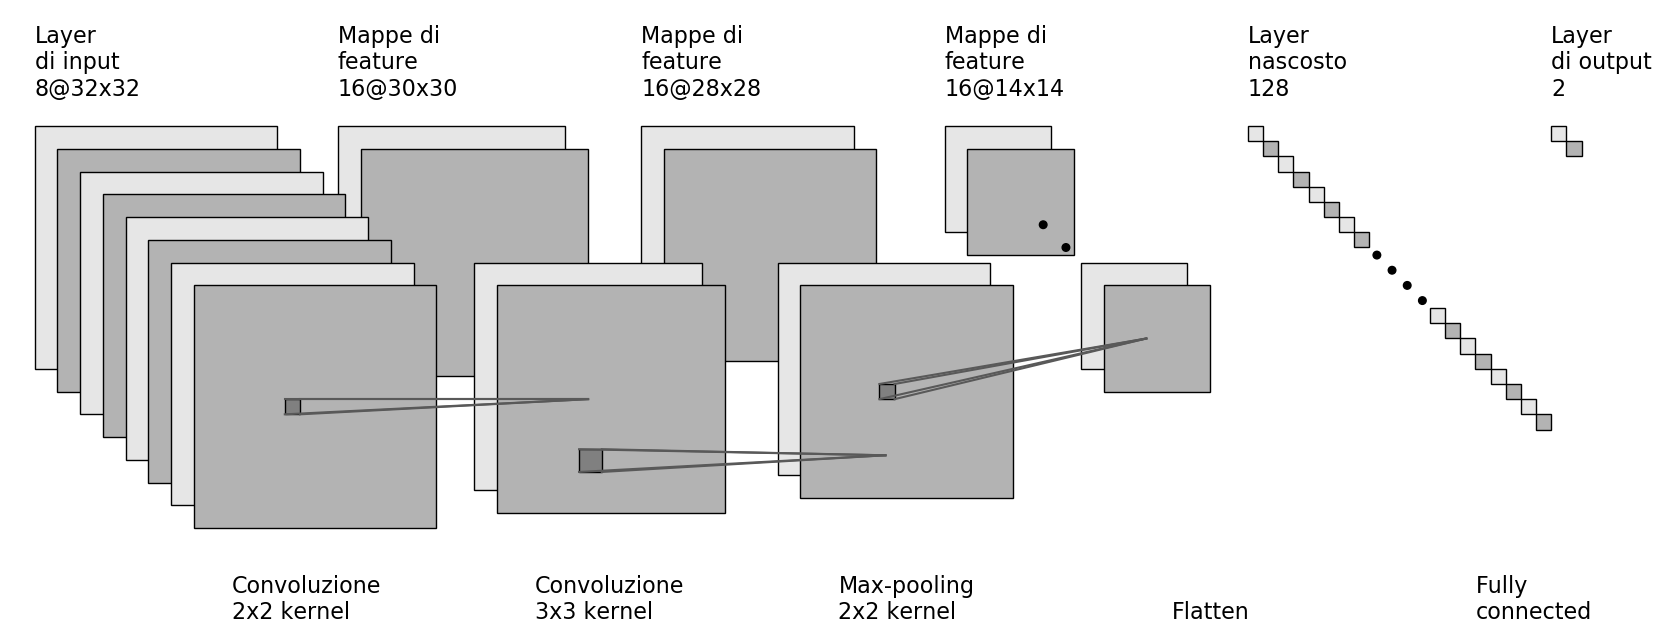
\includegraphics[scale=0.35]{cnn.png}}
 \label{fig:cnn}
 \caption{Schema di una rete convoluzionale effettivamente utilizzata per l'analisi di un sistema XY su reticolo $32\times32$, sono stati tralasciati i layer \emph{dropout}.}
\end{figure}

Il metodo migliore per classificare un modello XY risulta essere una rete convoluzionale \cite{melko}, uno schema di una rete di questo tipo effettivamente utilizzata in questo lavoro è rappresentato in Figura \ref{fig:cnn}.
Il layer di input può ricevere come argomento la semplice configurazione degli spin, quindi una matrice di valori reali nell'intervallo $[0,2\pi)$, oppure la configurazione espressa in vortici e antivortici, che appare come una matrice con valori $\{-1;0;+1\}$.


%----------------------------------------------------------------------------------------
%	SECTION 4
%----------------------------------------------------------------------------------------

\section{Risultati e conclusioni}

\subsection{Stima della temperatura critica}
Attraverso l'utilizzo delle reti neuronali, è stato possibile stimare la temperatura critica $T_c$ del modello di Ising, riportata nell'introduzione. Tale valore teorico è esatto per sistemi su reticolo di lato infinito; per sistemi di lato finito la temperatura critica presenta una correzione che aumenta al diminuire della dimensione del reticolo. Per stimare il valore teorico è stato effettuato il calcolo della temperatura critica su diversi reticoli al variare della lato del reticolo (in numero di spin) da $20$ a $90$, ogni $10$, andando poi ad interpolare i risultati e ottenendo il valore per $L\rightarrow \infty$.
%TODO provare a cercare la legge
La rete è stata allenata su set di almeno $100000$ configurazioni (prendendo un sottoinsieme di configurazioni pari al $10\%$ del training set per la validazione) a reticolo quadrato, e testata su set di $10000$ a reticolo sia triangolare che honeycomb: ciascun valore di temperatura riportato è dati dalla media di $10$ temperature, i cui valori sono classificati da $10$ diverse reti scelte in modo da avere una \emph{test accuracy} alta e una \emph{test loss} bassa. I parametri della rete sono riportati in tabella \ref{tab:ffnnpar}
\begin{table}[h]
\begin{center}
\begin{tabular}{llllllll}
\toprule
Rete & Layer & Neuroni & Batch size & w e b init & Attivazione & Earlystop & Rego\\
\midrule
FeedForward & $1$ & $100$ & $100$ & Random & Sigmoidale & si & L$2$ $0.01$\\
\bottomrule
\end{tabular}
\end{center}
\caption{Parametri}
\label{tab:ffnnpar}
\end{table}

\begin{figure}
\centering
\begin{tikzpicture}
\begin{axis}[
xlabel = {$L^{-1}$  [$\si{nspin}^{-1}$]}, 
ylabel={$T$ [\si{K}]},
grid=major,
major grid style={line width=.1pt, dashed, draw=gray!30},
]
\addplot[mark=none, red, thick] coordinates {(0.001,1.5187) (0.055,1.5187)};
\addlegendentry{Temperatura critica}
\addplot [only marks, blue]
plot [error bars/.cd, error bar style={red}, y dir = both, y explicit]
table [ y error index=2] {dati/honeycomb_pgf};
\addlegendentry{Temperatura} 
\end{axis} 
\end{tikzpicture}
\end{figure}
%----------------------------------------------------------------------------------------
%	BIBLIOGRAPHY
%----------------------------------------------------------------------------------------

\bibliographystyle{ieeetr}

\bibliography{relazione}

%----------------------------------------------------------------------------------------


\end{document}
